%   Modelo de trabalhos acadêmicos - IFRJ
%   Autor: Andrey Dione Ferreira - <andrey.ferreira@ifrj.edu.br>
%   Codificação utilizada: UTF-8
%   Tamanho da tabulação: 4 (espaços)
%	Atualizado em 03/06/2021

% \documentclass{ifrjtex}  % Imprimir frente e verso
\documentclass[oneside]{ifrjtex}  % Imprimir apenas frente

%-------------------------------------------------
% IMPORTAÇÃO DE PACOTES %
%-------------------------------------------------
\usepackage[T1]{fontenc} %Codificação da fonte em 8 bits
\usepackage{enumitem} %para customizar listas
\usepackage{smartdiagram} %Construção de diagramas
\usepackage[portuguese, onelanguage, lined, boxed, commentsnumbered, algoruled]{algorithm2e} % Escrever algoritmos
\usepackage{tikz,animate,pgfplots,multido} % Desenhar e fazer animações
\pgfplotsset{compat=1.16}
\usepackage{verbatim}     % Texto é interpretado como escrito no documento
\usepackage{multirow, array}    % Múltiplas linhas e colunas em tabelas
\usepackage{epstopdf}  % Faz a conversão de figuras.eps para pdf. Declarar a extensão de cada figura ao chamá-la


\usepackage[alf, abnt-emphasize=bf, recuo=0cm, abnt-etal-cite=2, abnt-etal-list=0]{abntex2cite}  % Citações padrão ABNT


% Criando novos comandos ou redefinindo outros
\renewcommand{\sin}{\mathrm{sen}}


\makeindex % Cria o índice remissivo


%------------------------------------------------
% PREENCHER COM OS DADOS DO TRABALHO            
%------------------------------------------------
\titulo{Título do trabalho}
%\title{Title in English}
\subtitulo{Subtítulo do trabalho}
\autor{Nome Completo do Autor}
\local{Volta Redonda}
\data{Janeiro de 2016}  % coloque a data de defesa no formato Mês de Ano
\instituicao{Instituto Federal de Educação, Ciência e Tecnologia do Rio de Janeiro}
\programa{Licenciatura em Matemática}
\preambulo{Trabalho de Conclusão de Curso submetido ao corpo docente do \imprimirinstituicao\, como requisito parcial para a obtenção do grau de Licenciado em Matemática.}
% \orientador{Nome do orientador}
\orientador[Orientadora:]{Nome da orientadora}
\titulacaoOrientador{Prof. Dr. }
\instOrientador{Instituto Federal do Rio de Janeiro - IFRJ}
\coorientador{Nome do coorientador}  % Caso não tenha, comente ou apague esta linha.
%\coorientador[Coorientadora:]{Nome da coorientadora}
\titulacaoCoorientador{Prof. Dr. }  % Caso não tenha, comente ou apague esta linha.
\instCoorientador{Instituto Federal do Rio de Janeiro - IFRJ}  % Caso não tenha, comente ou apague esta linha.
\date{2021} %Ano de defesa

%----------------------------------------------------
% DADOS PARA CATALOGAÇÃO:  CONSULTAR BIBLIOTECA DO CAMPUS APÓS DEFESA E CORREÇÃO
%----------------------------------------------------
\TabelaCutter{????}        % Preencher ???? com Tabela Cutter (Ver na biblioteca do campus)
\CDU{?????}      % Preencher com o código CDU (ver na biblioteca do Campus)
\keywords{ 1. Palavra-chave1. 2. Palavra-chave2. 2. Palavra-chave3.} %Preencher com as palavras chaves (Conferir na biblioteca do campus)
\sobrenomeAutor{ Sobrenome}   % Preencher com o último sobrenome do autor
\NomeAutor{Nome ... ...}   % Preencher com o nome do autor com exceção do último sobrenome
\sobrenomeOrientador{ Sobrenome ori }   % Preencher com o último sobrenome do orientador(a)
\NomeOrientador{Nome orientador}   % Preencher com o nome do orientador(a) com exceção do último sobrenome

%-------------------------------------------------
% INÍCIO DO DOCUMENTO
%------------------------------------------------
\begin{document}

\frenchspacing % Retira espaço extra obsoleto entre as frases
    
%-------------------------------------------------
% ELEMENTOS PRÉ-TEXTUAIS %
%-------------------------------------------------
    \pretextual
    \imprimircapa
    \imprimirfolhaderosto     % Folha de rosto
    % Documento: Ficha Catalográfica

\makeatletter
\begin{fichacatalografica}
	\sffamily
	\small
	\vspace*{\fill}
	\begin{center}
		\vspace{10pt}
		\fbox{
			{\RaggedRight 
			\begin{tabular}{l m{9.5cm}}
			& \\
			\imprimirTC & \imprimirautorultimo, \imprimirautornome \\
			&\ \ \ \  \imprimirtitulo  \,/ \imprimirautor, \thedate. \\			
			& \qquad \thelastpage p. : il.\\
			& \\
			& \qquad \imprimirorientadorRotulo~\imprimirTitulacaoOrientador~\imprimirorientador\\
			\abntex@ifnotempty{\imprimircoorientador}{%
            & \qquad\small\imprimircoorientadorRotulo~\imprimirTitulacaoCoorientador\, \imprimircoorientador\\}
			&Trabalho de Conclusão de Curso (\imprimirprograma ) ~--~\imprimirinstituicao, \thedate.\\
			& \\			
			& \qquad \imprimirorkeywords I. \imprimirorirultimo,\imprimirorientadornome. II. IFRJ. III. Título\\[0.5cm]
			\multicolumn{2}{l}{COBIB/CVOR {\hfill \imprimirCDU}}\\
			& \\
		\end{tabular}}
		}
		\end{center}
		\vspace*{\fill}
	\end{fichacatalografica}	
\makeatother
\cleardoublepage %ficha catalográfica
    % Documento: Folha de aprovação
\makeatletter
\begin{folhadeaprovacao}
\begin{center}
    {\large\fontfamily{cmr}\scshape\textbf\imprimirautor}
\end{center}
\vspace*{\fill}

\begin{center}
{\Large
\MakeUppercase{\imprimirtitulo}\abntex@ifnotempty{\imprimirsubtitulo}{{\MakeTextUppercase{: \imprimirsubtitulo}}
}}
\end{center}
\vspace*{\fill}

\begin{flushright}
\begin{minipage}{0.47\textwidth}
\SingleSpacing \small \imprimirpreambulo
\end{minipage}
\end{flushright}

\vspace*{\fill}

Aprovado em 01 de Janeiro de 2022
\vspace*{\fill}
        
\begin{center}
BANCA EXAMINADORA

    \assinatura{\textbf{\imprimirTitulacaoOrientador~\imprimirorientador} \\ Orientador/IFRJ}
    \abntex@ifnotempty{\imprimircoorientador}{
    \assinatura{\textbf{\imprimirTitulacaoCoorientador~\imprimircoorientador}\\ Co-Orientador/IFRJ}}
    
    \assinatura{\textbf{Professora} \\ Convidado 1/UFRJ}
    \assinatura{\textbf{Professor} \\ Convidado 2/UFF}
    \assinatura{\textbf{Professora} \\ Convidado 3}
    %\assinatura{\textbf{Professor} \\ Convidado 4}
\end{center}
\end{folhadeaprovacao}
\makeatother
     % Folha de aprovação
    %
% Documento: Dedicatória
%

\begin{dedicatoria}

Espaço reservado para dedicatória.
Inserir seu texto aqui... (OPCIONAL)

\end{dedicatoria}
         % Dedicatória (ELEMENTO OPCIONAL)
    %
% Documento: Agradecimentos
%

\begin{agradecimentos}

Inserir seu texto aqui...
(esta página é opcional)

\end{agradecimentos}
      % Agradecimentos  (ELEMENTO OPCIONAL)
    %
% Documento: Epígrafe
%

\begin{epigrafe}

\textit{``A minha vontade é forte, porém minha disposição de obedecer-lhe é fraca.'' (Carlos Drummond de Andrade)}

\end{epigrafe}
            % Epígrafe (ELEMENTO OPCIONAL)
    \include{elementos-pre-textuais/resumo-pt}           % Resumo na língua vernácula
    \include{elementos-pre-textuais/resumo-en}           % Resumo em língua estrangeira
    

    \pdfbookmark[0]{\listfigurename}{lof} \listoffigures*  \cleardoublepage  % Lista de figuras (OPCIONAL)
    \pdfbookmark[0]{\listfigurename}{log} \listofgraficos*  \cleardoublepage  % Lista de gráficos (OPCIONAL)
    \pdfbookmark[0]{\listtablename}{lot} \listoftables* \cleardoublepage      % Lista de tabelas (OPCIONAL)
    \pdfbookmark[0]{\listofquadrosname}{loq} \listofquadros* \cleardoublepage % Lista de quadros (OPCIONAL)
    
    %
% Documento: Lista de abreviaturas e siglas
%
\begin{siglas}
    \item[ABNT] Associação Brasileira de Normas Técnicas
    \item[IFRJ] Instituto Federal de Educação, Ciência e Tecnologia do Rio de Janeiro
\end{siglas}
        % Lista de abreviaturas e siglas (OPCIONAL)
    %
% Documento: Lista de símbolos
%

\begin{simbolos}
    \item[$ \Gamma $] Letra grega Gama
    \item[$ \lambda $] Comprimento de onda
    \item[$ \in $] Pertence
\end{simbolos}
      % Lista de símbolos (OPCIONAL)

%-------------------------------------------------
% Documento: Sumário
\pdfbookmark[0]{\contentsname}{toc}
\tableofcontents*
\cleardoublepage

%-------------------------------------------------
% ELEMENTOS TEXTUAIS %
%-------------------------------------------------
    \textual
    %
% Documento: Introdução
%
\chapter{Introdução}
\label{chap:introducao}

A classe \texttt{ifrjtex} consiste em uma extensão da classe \texttt{abn\TeX} e foi elaborada com o objetivo de facilitar a produção dos trabalhos acadêmicos do Instituto Federal de Educação, Ciência e Tecnologia do Rio de Janeiro por parte dos discentes e servidores da instituição, tratando-se de um projeto independente e não oficial.

Caso localize algum erro ou tenha sugestões de modificações, registre suas observações no \href{https://github.com/andrey-ferreira/ifrjTeX}{\textcolor{blue}{diretório do projeto}} ou entre em contato com o responsável pelo mesmo através do e-mail \href{mailto:andrey.ferreira@ifrj.edu.br}{\textcolor{blue}{andrey.ferreira@ifrj.edu.br}}.

Por se tratar de uma extensão {\ttfamily abntex2},  a constituição do documento torna-se facilitada, uma vez que o mesmo possui comandos especiais para auxiliar a distribuição/definição das diversas partes constituintes do projeto.
Esse estilo é baseado nas normas da ABNT\index{ABNT}.
Maiores detalhes relacionados aos comandos existentes no estilo poderão ser adquiridos através da documentação disponível no site \href{https://code.google.com/p/abntex2/}{https://code.google.com/p/abntex2/} \cite{abntex2classe}.

Uma das principais vantagens do uso do estilo de formatação para \LaTeX é a formatação \textit{automática} dos elementos que compõem um documento acadêmico, tais como capa, folha de rosto, dedicatória, agradecimentos, epígrafe, resumo, abstract, listas de figuras, tabelas, siglas e símbolos, sumário, capítulos, referências, etc.

Neste documento o leitor encontrará instruções específicas para o uso da classe \texttt{ifrjtex} e poucas instruções sobre a escrita de alguns elementos textuais em \LaTeX. 

Para melhor entendimento do uso do estilo de formatação, aconselha-se que o potencial usuário analise os comandos existentes no arquivo {\ttfamily main.tex} e os resultados obtidos no arquivo {\ttfamily main.pdf} depois do processamento pelo software \LaTeX  \cite{LaTeX2009}.
Recomenda-se a consulta ao material de referência do software para a sua correta utilização \cite{Lamport1986,Buerger1989,Kopka2003,Mittelbach2004}.            % Introdução
    %
% Documento: Trabalhos Relacionados
%
\chapter{Uso do modelo}

Por se tratar de uma extensão da classe \verb|abntex2|, todas as opções, ambientes e macros da classe \verb|abntex2|\cite{abntex2classe}
e \verb|memoir|\cite{madsen2021memoir} podem ser utilizadas.


\section{Opções para a classe \texttt{ifrjtex}}

As opções \verb|artigo| e \verb|projeto| podem ser passadas ao carregar a classe para que a folha de rosto seja ajustada automaticamente ao formato exigido pelo Manual de Apresentação de Trabalhos Acadêmicos \cite{ifrjtccs}.

Caso o usuário opte por editar estes elementos, recomendamos que seja redefinida as macros específicas para a impressão dos mesmos fornecidas pela \verb|abntex2|\cite{abntex2classe}.

\subsection{Projetos de Pesquisa}
Conforme definido no Manual de Apresentação de Trabalhos Acadêmicos, a estrutura de um projeto podem variar conforme as normas estabelecidas pela instituição.
\begin{citacao}
O projeto de pesquisa é um planejamento das etapas do trabalho que será desenvolvido. Sua estrutura pode variar de acordo com as normas estabelecidas pela instituição, sendo constituído pela parte externa e pela parte interna. A externa constitui-se de capa (obrigatória), e a interna é organizada por elementos pré-textuais, elementos textuais e elementos pós-textuais.\cite{ifrjtccs}
\end{citacao}

Para que o modelo imprima os elementos pré-textuais com os elementos exigidos no Manual, a opção \verb|projeto| pode ser passada à classe quando a mesma for selecionada, conforme segue.

\textbackslash\texttt{documentclass[projeto]\{ifrjtex\}}

No entanto, ao construir este modelo em \LaTeX, o autor disponibilizou, além dos elementos exigidos, a macro \verb|\areaconcentracao{}|, visto que muitos programas podem exigir entregas de projetos vinculados à áreas de concentração ou linhas de pesquisa, por exemplo. Dessa forma, optou-se por imprimir na folha de rosto a entrada da macro \verb|\areaconcentracao{}| caso esta seja preenchida.

Os dados da macro \verb|\areaconcentracao{}| são impressos por padrão na folha de rosto após o preâmbulo com o rótulo ``\textbf{Área de concentração: }''.

Caso o usuário queira modificar esse rótulo, pode-se passar um novo rótulo como opção para a macro \verb|\areaconcentracao{}|. Por exemplo, se no preâmbulo o usuário substituir \verb|\areaconcentracao{Nome da área de concentração}| por \\ \verb|\areaconcentracao[Linha de pesquisa: ]{Nome da linha}|, será impresso o rótulo ``\textbf{Linha de pesquisa: }'' no lugar de ``\textbf{Área de concentração: }''.

\subsection{Artigos}
Segundo orientações do Manual de Apresentação de Trabalhos Acadêmicos
\begin{citacao}
Os autores dos artigos submetidos em periódicos externos e de acesso livre, que utilizaram esse tipo de publicação como TCC, deverão comunicar à
Biblioteca do campus onde cursaram sobre a existência da pesquisa, enviando uma cópia do artigo para depósito no repositório institucional (RI) do IFRJ, observando a obrigatoriedade da utilização dos seguintes elementos pré- textuais:\\
    a) capa: elemento obrigatório, deverá ser feita conforme o modelo no Apêndice A e o especificado na seção 2.1;\\
    b) folha de rosto: elemento obrigatório, contém os elementos essenciais à identificação do artigo, de acordo com Apêndice E;\\
   c)verso da folha de rosto: elemento obrigatório, contém a ficha catalográfica confeccionada obrigatoriamente por um bibliotecário da Instituição;\\
    d)folha de aprovação: elemento obrigatório, contém os elementos essenciais à aprovação do trabalho. Após a assinatura da banca, a folha deve ser digitalizada e inserida no documento digital. \cite{ifrjtccs}
\end{citacao}

Para que o modelo imprima esses elementos em conformidade com o Manual, a opção \verb|artigo| pode ser passada à classe quando a mesma for selecionada, conforme segue.

\textbackslash\texttt{documentclass[artigo]\{ifrjtex\}}

Para inserção do artigo submetido em periódicos externos e de acesso livre, recomendamos que o autor utilize após a folha de aprovação o comando \\ \noindent\verb|\includepdf[pages=-]{myfile.pdf}| fornecido pelo pacote \verb|pdfpages| \cite{pdfpages}.




\section{Referências bibliográficas e citações}

Nesta versão da classe, optamos por utilizar o tratamento das referências bibliográficas com o {\ttfamily biblatex} e o estilo \texttt{abnt}, visto que
\begin{citacao}
Sendo totalmente implementado em \LaTeX, ele substitui os arquivos de estilo \verb|bibtex abntex2-alf.bst, abntex2-num.bst| e o pacote \verb|abntex2cite.sty| descrito neste manual. Com isso, o \verb|biblatex-abnt| deve aposentar os estilos de formatação do \verb|abntex2cite| e utilizar exclusivamente o \verb|biblatex-abnt| e as macros padrões do Bib\LaTeX. \cite{araujopacote}
\end{citacao}

Recomendamos que seja lida as referências específicas dos pacotes \verb|biblatex-abnt| disponíveis em \url{https://www.ctan.org/pkg/biblatex-abnt}.

Conforme orientado por \textcite{marquesbiblatex}, o \verb|biblatex-abnt 3.4| requer \verb|biblatex 3.8| e \verb|biber 2.8| e caso haja algum problema na compilação, cheque se seus pacotes estão atualizados.

Exemplos de entrada para o \verb|biblatex|, semelhantes aos encontrados no arquivo \verb|refbase.bib| deste projeto, podem ser encontradas em \textcite{marquesbiblatex} e todas as possíveis entradas, distinguindo entre campos obrigatórios e opcionais podem ser consultadas em \cite{lehman2006biblatex}. Além disso, todas as saídas geradas conforme a NBR 10520:2002 usando o sistema autor-data podem ser consultadas em \textcite{marquesexemplos}.

Recomenda-se ainda que o potencial usuário deste modelo utilize gerenciadores de bases bibliográficas como o \textcite{JabRef2009} e \textcite{Zotero}.

\subsection{Citações livres}\label{citacoesLivres}
Citações são trechos transcritos ou informações retiradas das publicações consultadas para a realização do trabalho.
As citações são utilizadas no texto com o propósito de esclarecer, completar, embasar ou corroborar as ideias do autor.

Todas as publicações consultadas e efetivamente utilizadas (através de citações) devem ser listadas, obrigatoriamente, nas referências bibliográficas, de forma a preservar os direitos autorais e intelectuais.

Na utilização de citações, normalmente, utiliza-se referências.
Para cada tipo de referência presente no texto será apresentado um exemplo do comando utilizado para criá-lo.

Há basicamente dois tipos de citações: citações livres e citações literais.

Nas citações livres, reproduzem-se as ideias e informações de um autor, sem, entretanto, ``copiar letra por letra'' o texto do autor.
Há várias maneiras de se fazer uma citação livre, como mostra os exemplos abaixo.

Por outro lado, \textcite{maturana:2003} defende um princípio de lógica.
Para o autor, quando dizemos \ldots

Além disso, \textcite{teste:2004} argumenta que \ldots\mbox{ }Observe o detalhe do termo \textit{et al}.
que deve ser utilizado quando o trabalho citado possui mais de três autores.
Esse recurso é automatizado pelo estilo {\ttfamily abntex2}\index{ABNT!abntex2}.
Caso não haja desejo em abreviar o nome dos demais autores através do termo \textit{et al.}, deve-se incluir a opção {\ttfamily abnt-no-etal-label}.

Para evitar uma interrupção na sequência do texto, o que poderia, eventualmente, prejudicar a leitura, pode-se indicar a fonte entre parênteses imediatamente após a citação livre.
Porém, neste caso específico, o nome do autor deve vir em caixa alta, seguido do ano da publicação, como no exemplo a seguir.

\cite{BibTeX2009}

\subsection{Citações literais}\label{citacoesLiterais}
Nas citações literais, reproduzem-se as ideias e informações de um autor, exatamente como este a expressou, ou seja, faz-se uma ``cópia letra por letra'' do texto do autor.
Há várias maneiras de se fazer uma citação literal, como mostra os exemplos abaixo.

As citações longas (mais de 3 linhas) devem usar um parágrafo específico para ela, na forma de um texto recuado (4 cm da margem esquerda), com tamanho de letra menor do aquela utilizada no texto e espaçamento simples entre as linhas, seguido dos sobrenomes dos autores em caixa alta (separados por ponto e vírgula), ano de publicação e número da página.
Veja o exemplo abaixo.

\begin{citacao}
Desse modo, opera-se uma ruptura decisiva entre a reflexividade filosófica, isto é a possibilidade do sujeito de pensar e de refletir, e a objetividade científica.
Encontramo-nos num ponto em que o conhecimento científico está sem consciência.
Sem consciência moral, sem consciência reflexiva e também subjetiva.
Cada vez mais o desenvolvimento extraordinário do conhecimento científico vai tornar menos praticável a própria possibilidade de reflexão do sujeito sobre a sua pesquisa \cite[p.28]{morinmoigne:2000}.
\end{citacao}

Para se criar o efeito demonstrado na citação anterior, deve-se utilizar o ambiente \texttt{citacao}.
\begin{verbatim}
\begin{citacao}
    Desse modo, opera-se uma ruptura decisiva entre a reflexividade
    filosófica, isto é a possibilidade do sujeito de pensar e de refletir,
    e a objetividade científica. Encontramo-nos num ponto em que o 
    conhecimento científico está sem consciência.
    Sem consciência moral, sem consciência reflexiva e também subjetiva.
    Cada vez mais o desenvolvimento extraordinário do conhecimento 
    científico vai tornar menos praticável a própria possibilidade 
    de reflexão do sujeito sobre a sua pesquisa \cite[p.28]{morinmoigne:2000}.
\end{citacao}
\end{verbatim}

Opcionalmente, pode-se referenciar os autores no corpo de texto (neste caso seus nomes devem vir em minúsculas), e em seguida colocar a citação literal, em um novo parágrafo recuado.
Note que pode após a citação literal não mais aparece o nome dos autores, visto que já se encontra no texto.
Veja o exemplo seguinte.

\textcite[p.~33]{morinmoigne:2000}, ao fazerem as suas críticas à ciência, explicitam uma ideia coletiva:

\begin{citacao}
Mas o curioso é que o conhecimento científico que descobriu os meios realmente extraordinários para, por exemplo, ver aquilo que se passa no nosso sol, para tentar conceber a estrutura das estrelas extremamente distantes, e até mesmo para tentar pesar o universo, o que é algo de extrema utilidade, o conhecimento científico que multiplicou seus meios de observação e de concepção do universo, dos objetos, está completamente cego, se quiser considerar-se apenas a si próprio!
\end{citacao}

As citações curtas (menos de 3 linhas) devem ser inseridas diretamente no texto (entre aspas), seguida do nome do autor (em caixa alta), ano e página, como no exemplo a seguir.

Então significa apenas que ``assumo que não posso fazer referência a entidades independentes de mim para construir meu explicar'' \cite[p.~35]{maturana:2003}.

O conhecimento de \textcite[p.~35]{maturana:2003} aponta que isto significa apenas que ``assumo que não posso fazer referência a entidades independentes de mim para construir meu explicar''.

Finalmente, e isto vale para citações curtas ou longas, caso seja necessário inserir, no meio de uma citação uma palavra ou frase curta de sua autoria, que sirva para clarear ou completar a frase do autor citado, isto deve ser feito colocando a citação entre aspas.
O comentário deverá ser inserido sem aspas.
Ou seja, todo texto da citação deverá ficar envolvido por aspas.
O exemplo abaixo apresenta o resultado esperado.

Significa apenas que ``assumo que não posso fazer referência a entidades'' objetivas no sentido tradicional ``independentes de mim para construir meu explicar'' {\textcite[p.~35]{maturana:2003}}.

\subsection{Comandos para citações}\label{referenciasUtilizadas}

Alguns exemplos de citação conforme \textcite{marquesbiblatex}:

\begin{itemize}
    \item \textcite{maturana:2003}\\ \verb|\textcite{maturana:2003}|
    \item \textcite{teste:2004}\\ \verb|\textcite{teste:2004}|
    \item \cite[p.~28]{morinmoigne:2000}\\ \verb|\cite[p.~28]{morinmoigne:2000}|
    \item \textcite[p.~33]{morinmoigne:2000}\\ \verb|\textcite[p.~33]{morinmoigne:2000}|
    \item \cite[p.~35]{maturana:2003}\\ \verb|\cite[p.~35]{maturana:2003}|
    \item \textcite[p.~35]{maturana:2003}\\ \verb|\textcite[p.~35]{maturana:2003}|
    \item \cite{teste:2004,maturana:2003}\\ \verb|\cite{teste:2004,maturana:2003}|
    \item \apud{maturana:2003}{morinmoigne:2000}\\
    \verb|\apud{maturana:2003}{morinmoigne:2000}|
\end{itemize}


%
% Documento: Fundamentação Teórica
%

\chapter{Elementos flutuantes, equações e referências cruzadas}
\label{chap:ef}

\textcolor{red}{\large ESTE CAPÍTULO SERÁ ATUALIZADO COM ORIENTAÇÕES DE USO DE MELHORES PACOTES!!}

A seguir ilustra-se a forma de incluir figuras, tabelas, equações, siglas e 
símbolos no documento, obtendo indexação automática em suas respectivas
                listas.
A numeração sequencial de figuras, tabelas e equações ocorre de modo automático.
Referências cruzadas são obtidas através dos comandos \verb#\label{}# e \verb#\ref{}#.
Por exemplo, não é necessário saber que o número deste capítulo é \ref{chap:ef} para colocar o seu número no texto.
Isto facilita muito a inserção, remoção ou relocação de elementos numerados no texto (fato corriqueiro na escrita e correção de um documento acadêmico) sem a necessidade de renumerá-los todos.





 
\section{Equações}
\label{sec:equacoes}

A transformada de Laplace é dada na \autoref{eq:laplace}, enquanto a \autoref{eq:dft} apresenta a formulação da transformada discreta de Fourier bidimensional\footnote{Deve-se reparar na formatação esteticamente perfeita destas equações.}.


\begin{equation}
    X(s) = \int\limits_{t = -\infty}^{\infty} x(t) \, \text{e}^{-st} \, dt
    \label{eq:laplace}
\end{equation}

\begin{equation}
    F(u, v) = \sum_{m = 0}^{M - 1} \sum_{n = 0}^{N - 1} f(m, n) \exp \left[ -j 2 \pi \left( \frac{u m}{M} + \frac{v n}{N} \right) \right]
    \label{eq:dft}
\end{equation}


\section{Elementos flutuantes (tabelas, quadros, gráficos e figuras)}

Tabelas, quadros, gráficos e figuras são elementos utilizados em trabalhos acadêmicos, e possuem diferenças e especificações definidas pela ABNT.

As tabelas são formadas por linhas verticais, devem manter suas bordas laterais abertas e geralmente são utilizadas para dados quantitativos. Os quadros, por outro lado, são formados por linhas verticais e horizontais, devem ter todas suas extremidades fechadas e são mais utilizados para dados qualitativos.

Por último, as figuras e gráficos são elementos ilustrativos, que podem ser em forma de fotos, mapas, gráficos, gravuras, etc.

Todos estes elementos devem estar centralizados, com legenda na parte superior e fonte na parte inferior (ver Quadro \ref{quadroex1} para maiores detalhes).

De forma geral, esses ambiantes podem ser utilizados com os seguintes comandos



\begin{verbatim}
\begin{nome do ambiente}[H]
   \centering
   \caption{legenda}
   \label{"etiqueta"}
      inserção do elemento 
   \fonte{fonte do elemento}
\end{table}
\end{verbatim}
Os campos apresentados nos códigos acima estão explicados no Quadro \ref{quadroex2}.


\begin{quadro}[H]
	\centering
	\caption{Alguns detalhes sobre elementos flutuantes}
	\label{quadroex1}
	\begin{tabular}{|l|m{4cm}|m{4cm}|m{4cm}|}
		\hline
		& \textbf{Tabela}                                                                             & \textbf{Quadro}                                                                             & \textbf{Figuras}                                                                    \\ \hline
		\textbf{Formato}    & Bordas laterais não podem ser fechadas.                                                     & As extremidades devem ser fechadas.                                                         & Podem ser em forma de fotos, mapas, gráficos, gravuras, etc.                        \\ \hline
		\textbf{Uso}        & Geralmente para dados quantitativos.                                                        & Geralmente para dados qualitativos.                                                         & Ilustrar informações e dados.                                                       \\ \hline
		\textbf{Elementos}  & Título, cabeçalho, conteúdo, fonte e, se necessário, notas explicativas.                    & Título, fonte, legenda e notas.                                                             & Título, numeração e fonte.                                                          \\ \hline
		\textbf{Divisão}    & Formada por linhas verticais.                                                               & Formado por linhas horizontais e verticais.                                                 & -                                                                                   \\ \hline
		\textbf{Formatação} & O número e o título da tabela devem vir acima dela, enquanto a fonte deve aparecer embaixo. & O número e o título do quadro devem vir acima dele, enquanto a fonte deve aparecer embaixo. & O número e o título devem aparecer no topo, enquanto a fonte deve aparecer embaixo. \\ \hline
	\end{tabular}
	\fonte{\textcite{diana}}
\end{quadro}

\begin{quadro}[H]
	\centering
	\caption{Alguns campos utilizados em elementos flutuantes}
	\label{quadroex2}
	\begin{tabular}{|m{4cm}|m{8cm}|}
		\hline
	\verb|nome do ambiente| & \verb|figure|: para figuras, \verb|grafico|: para gráficos, \verb|table|: para tabelas e \verb|quadro|: para quadros\\ \hline
	\verb|legenda| & Deve ser inserida como argumento no comando \verb|\caption{}| e refere-se a legenda do elemento flutuante.\\ \hline
	\verb|"etiqueta"| & Deve ser inserida como argumento no comando \verb|\label{}| e consiste em um nome dado para referenciarmos àquele elemento flutuante no texto.\\ \hline
	\verb|fonte do elemento| & Deve ser inserida como argumento no comando \verb|\fonte{}| e consiste da informação de onde retirou-se o elemento.\\ \hline
	\end{tabular}
	\fonte{Elaborado pelo autor}
\end{quadro}


Abaixo apresentamos alguns exemplos de outros elementos flutuantes  seguidos dos códigos utilizados para inseri-los.

A Figura \ref{fig:conceitodt} aparece automaticamente na lista de figuras.
Para uso avançado de imagens no \LaTeX, recomenda-se a consulta de literatura especializada \cite{Goossens2007}.

\begin{figure}[H]
	\centering
	\caption{Ilustração do conceito de derivada topológica.}
	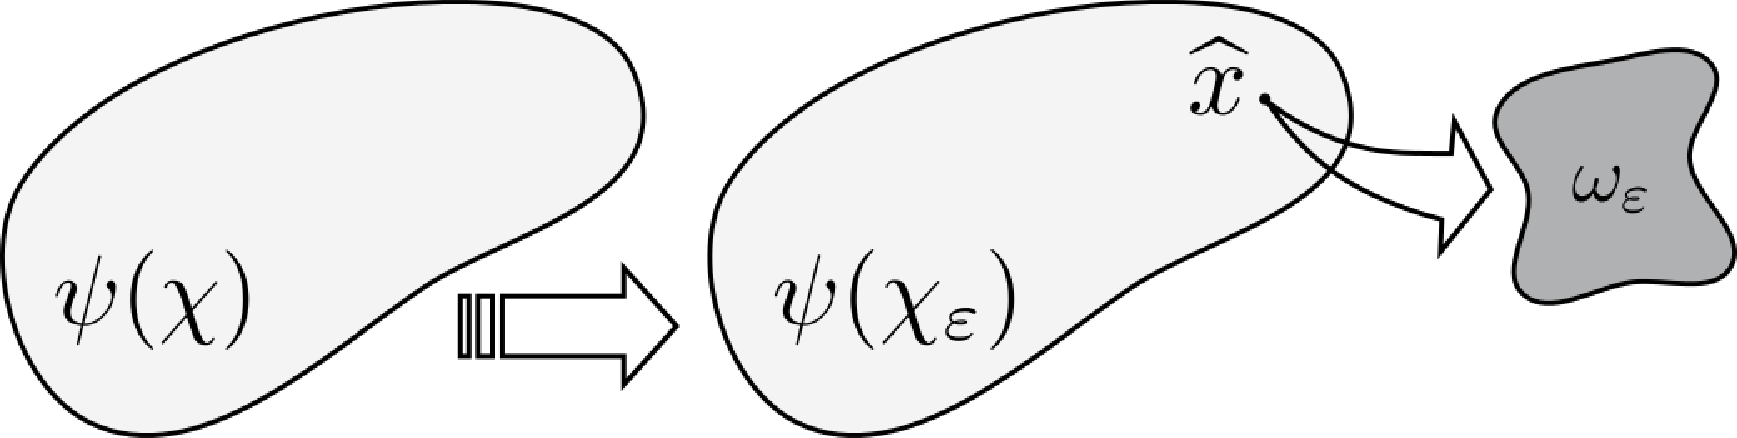
\includegraphics[width=0.6\textwidth]{./figuras/conceito.pdf}
	\fonte{\textcite{NovotnyBook2013}}
	\label{fig:conceitodt}
\end{figure}

\begin{verbatim}
\begin{figure}[H]
  \centering
  \caption{Conceito de derivada topológica.}
    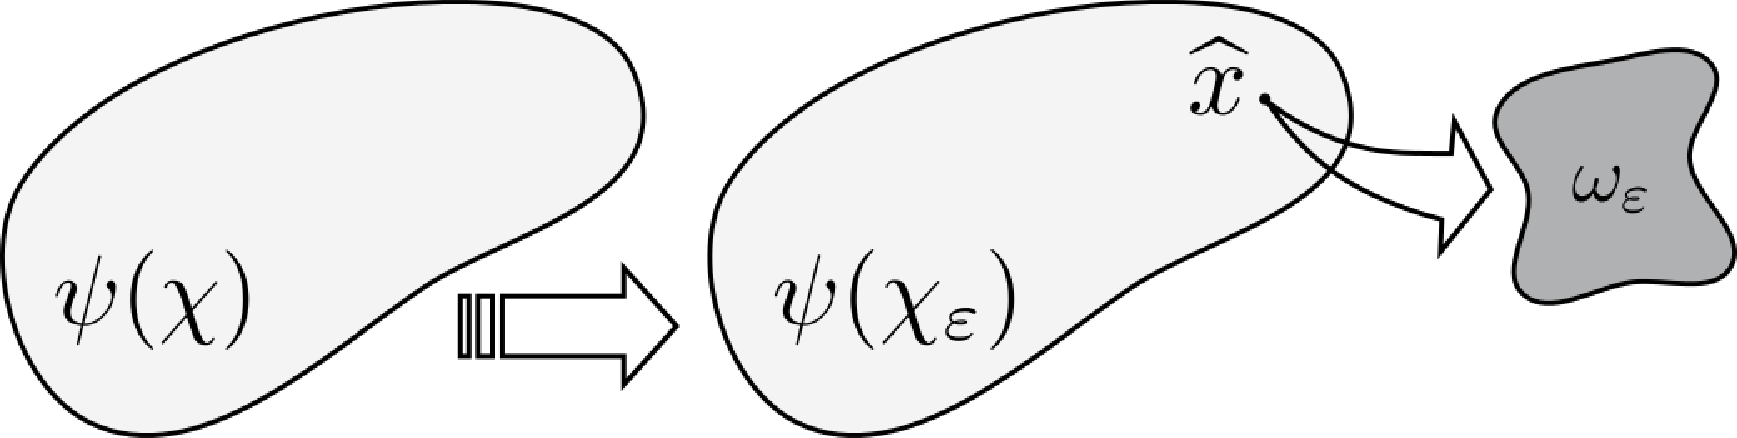
\includegraphics[width=0.6\textwidth]{./figuras/conceito.pdf}
  \fonte{\textcite{NovotnyBook2013}}
  \label{fig:conceitodt}
\end{figure}
\end{verbatim}


\begin{table}[H]
\centering
\caption{Um nome qualquer}
\label{ExemploTab}
\begin{tabular}{r|lr}	
Posição & País & IDH \\ \hline
	1 & Noruega        & .955 \\
	2 & Austrália  & .938 \\
	3 & EUA            & .937 \\
	4 & Holanda        & .921 \\
	5 & Alemanha       & .920            % não é preciso quebrar a última linha
\end{tabular}
% \fonte{\textcite{garcia}}
\end{table}

\begin{verbatim}
\begin{table}[H]
\centering
\caption{Um nome qualquer}
\label{ExemploTab}
\begin{tabular}{r|lr}	
    	Posição & País & IDH \\	\hline
    	1 & Noruega        & .955 \\
    	2 & Austrália  & .938 \\
    	3 & EUA            & .937 \\
    	4 & Holanda        & .921 \\
    	5 & Alemanha       & .920 
\end{tabular}
\fonte{\textcite{garcia}}
\end{table}
\end{verbatim}


\pagebreak

No Gráfico \ref{gr:exgrafico} apresentamos um exemplo de gráfico.

\begin{grafico}[H]
\centering
\caption{Evolução de matrículas dos Institutos Federais}
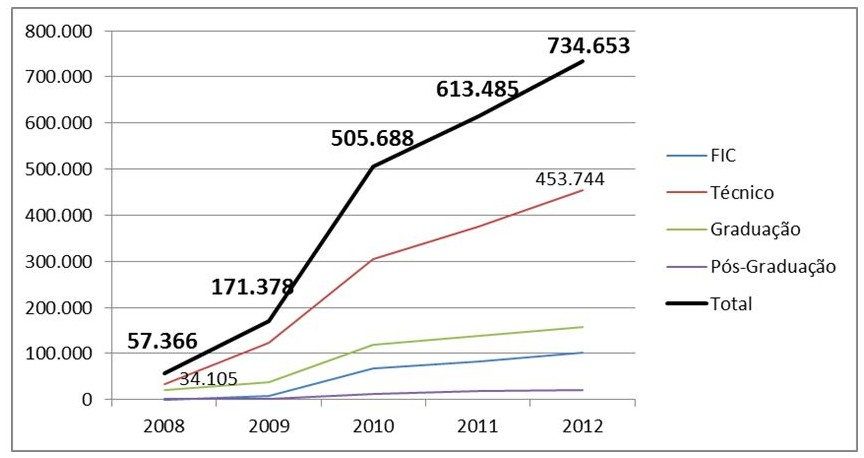
\includegraphics[height=6cm]{./figuras/redefederal.jpg}	
\fonte{MEC/SETEC}
\label{gr:exgrafico}
\end{grafico}

\begin{verbatim}
\begin{grafico}[H]
  \centering
  \caption{Evolução de matrículas dos Institutos Federais}
    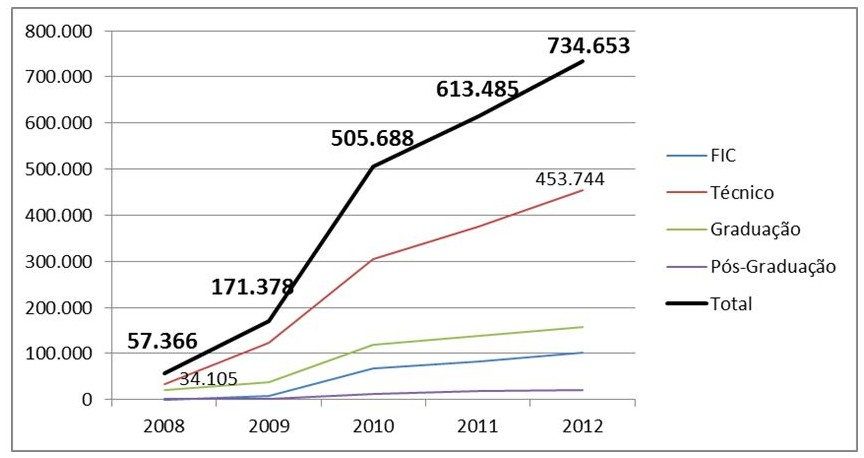
\includegraphics[height=6cm]{./figuras/redefederal.jpg}	
  \fonte{MEC/SETEC}
  \label{gr:exgrafico}
\end{grafico}
\end{verbatim}
    %
% Documento: Conclusão
%

\chapter{Considerações finais}
\label{chap:Considerações finais}


Espera-se que o uso do estilo de formatação \LaTeX\, adequado às Normas para Elaboração de Trabalhos Acadêmicos do IFRJ ({\ttfamily ifrjtex.cls}) facilite a escrita de documentos no âmbito desta instituição e aumente a produtividade de seus autores. Para usuários iniciantes em \LaTeX, além da bibliografia especializada já citada, existe ainda uma série de recursos \cite{CTAN2009} e fontes de informação \cite{TeX-Br2009,Wikibooks2009} disponíveis na Internet.

Recomenda-se o uso de um gerenciador de referências como o Mendeley \cite{Mendeley2009} ou JabRef\index{JabRef} \cite{JabRef2009}  para a catalogação bibliográfica em um arquivo BIBTEX, de forma a facilitar citações através do comando \verb#\cite{}# e outros comandos correlatos do pacote ABNTEX. A lista de referências deste documento foi gerada automaticamente pelo software \LaTeX + BIBTEX a partir do arquivo {\ttfamily refbase.bib}, que por sua vez foi composto com o gerenciador de referências Mendeley.
             % Conclusão

%-------------------------------------------------
% ELEMENTOS PÓS-TEXTUAIS %
%-------------------------------------------------
    \postextual
    \bibliography{./refbase}    % Geração automática das referências por meio do arquivo 'refbase.bib'
    % \printbibliography % Geração automática das referências por meio do arquivo 'refbase.bib'
    %
% Documento: Apêndices
%

\begin{apendicesenv}
\partapendices

\chapter{Nome do Apêndice}
\label{chap:apendicea}

Inserir seu texto aqui...



\chapter{Nome do Apêndice}
\label{chap:apendiceb}

Inserir seu texto aqui...


\end{apendicesenv}
   % Apêndices
    %
% Documento: Anexos
%

\begin{anexosenv}
\partanexos

\chapter{Nome do Anexo}
\label{chap:anexox}

Inserir seu texto aqui...


\end{anexosenv}
  % Anexos
  
    \printindex  % Imprimie o índice remissivo
\end{document}
